\chapter{Stand des Wissens und der Technik}
Für den Grundaufbau der Messmethodik ist das Grundwissen über einzelne Elemente unverzichtbar. In diesem Kapitel wird auf spezifisch ausgewählte Punkte eingegangen, um das Verständnis weiterer Zusammenhänge für den Leser zu vereinfachen.


\section{Funktionsweise eines Prozessors}

Ein Prozessor ist eine universelle Rechenmaschine, die sich durch eine definierte Reihe von Anweisungen programmieren lässt. Zu den arithmetischen Anweisungen gehören der Zugriff auf Speicheradressen und Sprünge innerhalb der Abfolge der Anweisungen.
Bereits der britische Mathematiker Alan Turing konnte aufzeigen, dass ein universelles Berechnungsmodell umsetzbar ist, wenn ein Rechner neben dem Speicherzugriff auch Sprünge besitzt\cite{Hoffmann2014l}. Auf diesen besonderen Eigenschaften bauen die heutigen Prozessoren auf. Ein Programm, das den Prozessor ansteuert, besteht aus einer endlichen Anzahl von geordneten Anweisungen. Der Prozessor befolgt, streng nach dem Ablauf, Anweisung für Anweisung. Diese ablaufenden Anweisungen können dabei auch Sprünge zu anderen Stellen innerhalb des Programms definieren.
\par
Die Prozessoren, auch Zentraleinheiten oder CPUs genannt, besitzen im Inneren drei Einheiten, die über einen Datenbus verbunden sind. Dies ist in der \autoref{fig:CPU} ersichtlich. Dabei kann der Datenbus je nach Grösse oder Leistung der CPU variieren. Die zurzeit meist verbreiteten CPUs, die in PCs verbaut sind, verwenden einen 64bit-Datenbus. In dieser Arbeit wird aber mit kleineren CPUs, die lediglich einen 32bit-Datenbus besitzen, gearbeitet. Die Control Unit\cite{patterson2013computer} ist dafür verantwortlich, dass das Programm immer an der richtigen Stelle ausgeführt wird. Sie nimmt Anweisungen an, dekodiert diese und übergibt sie der Arithmetic Logic Unit (ALU). Die Übergabe der Daten an die ALU und die Register erfolgt durch die Weichenstellung des Datenbusses. Die ALU ermöglicht es, Rechen- sowie logische Operationen an den Daten auszuführen. Die Register haben die Grösse des Datenbusses und dienen dazu, die Daten von und zur ALU zu bewegen. Eine CPU besitzt mehrere Register, die je nach CPU-Architektur variieren. Die Register lassen sich in zwei Kategorien, Universal- und Hilfsregister, unterteilen. In den Universalregistern lassen sich die zu bearbeitenden Daten speichern. Die Hilfsregister haben je nach ihrer Funktion eine besondere Rolle zugeordnet erhalten. Beispielsweise zählt das Statusregister zu den Hilfsregistern. Dieses spezielle Hilfsregister gibt Aufschluss über das Resultat der vorherigen Operation. So lässt sich über dieses Hilfsregisters herauslesen, ob eine Operation von zwei Zahlen den möglichen Speicherplatz des Registers übersteigt und es zu einem sogenannten "overflow" kommt.
Da die Anzahl Universalregister meist sehr klein ist, müssen die Daten immer wieder von den Universalregistern in den RAM und zurückgeladen werden.



\begin{comment}
Useful example for Pipelining

It may take X hours to build a single car, but if you start building a car then 30 seconds later start building another and every 30 seconds start another then after X hours you will have a new car every 30 seconds. Does that mean it takes 30 seconds to make a car? Of course not. But it does mean that once up and running you can average a new car every 30 seconds on that production line.

More info:
https://books.google.ch/books?id=PSonZP4Nj5sC&pg=PA11&lpg=PA11&dq=raspberry+half+cpu+cycle&source=bl&ots=m_3q-usqla&sig=Ub9KeDbuSkCLgFGSRyFc_KZs7Ow&hl=en&sa=X&ved=0ahUKEwj89Pa6iZnNAhXEiRoKHRtUALcQ6AEIMTAC#v=onepage&q=raspberry%20half%20cpu%20cycle&f=false
\end{comment}



\begin{figure}[t]
\centering
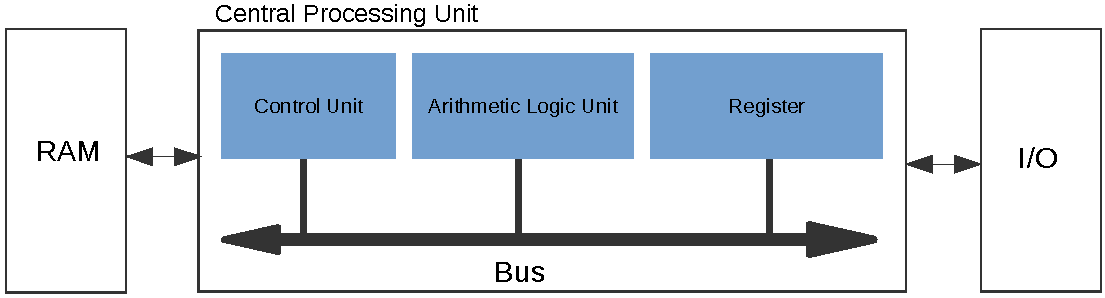
\includegraphics[width=1.0\textwidth]{images/cpu.pdf}
\caption{Central Processing Unit}
\label{fig:CPU}
\end{figure}

\section{Aufbau des Linux Betriebssystems}
% Monolithische Systeme 
% TRAP-Instruktion

Durch das Betriebssystem Minix, das von Andrew S. Tanenbaum für Ausbildungszwecke erstellt wurde, inspiriert, machte es sich Linus Torvalds zum Ziel, dieses vollwertige System neu zu schreiben. Im Jahr 1991 erschien die erste Linux Version 0.01\cite{ehses2011systemprogrammierung_chap2}. Heute ist es ein weit verbreitetes Betriebssystem, das für unterschiedlichen Anwendungszwecke wie für Desktops, Server, Smartphones und Embedded Systems eingesetzt wird.
\par
Die Aufgabe des Betriebssystemkerns, der meistens einfach nur Kernel genannt wird, ist es, eine Softwareschicht zwischen Hardware und Programm zu erstellen. Die Programme haben somit keinen direkten Zugriff auf die Hardware. Jedes Programm, das Informationen der Hardware benötigt, muss durch die Schicht des Kernels gehen. Die Kommunikationen zwischen Programm und Kernel werden Systemaufrufe (engl. Systemcalls) genannt. Die unterschiedlichen Systemaufrufe sind im POSIX standardisiert\cite{ehses2011systemprogrammierung_chap2}. Zusätzlich erstellt der Kernel eine Art Abkapselung eines Programms. Dadurch können mehrere Programme gleichzeitig laufen, ohne dass das eine Programm Zugriff auf das andere hat. Der Kernel verteilt die freien Ressourcen der CPU abwechslungsweise an die Programme. Dieses Verfahren heisst Multitasking und wurde seit den Anfängen unterstützt.
\par
Durch die zusätzliche Softwareschicht, die der Kernel bietet, müssen Programmierer ein Programm nicht für eine bestimmte Hardware schreiben, sondern für ein bestimmtes Betriebssystem. Dies ermöglicht eine höhere Portabilität eines Programms. Hardware wie Festplatten oder Netzwerkcontroller werden vom Kernel vereinheitlicht und dem Programm durch Systemaufrufe zur Verfügung gestellt.
\par

\begin{wrapfigure}{L}{0.49\textwidth}
\centering
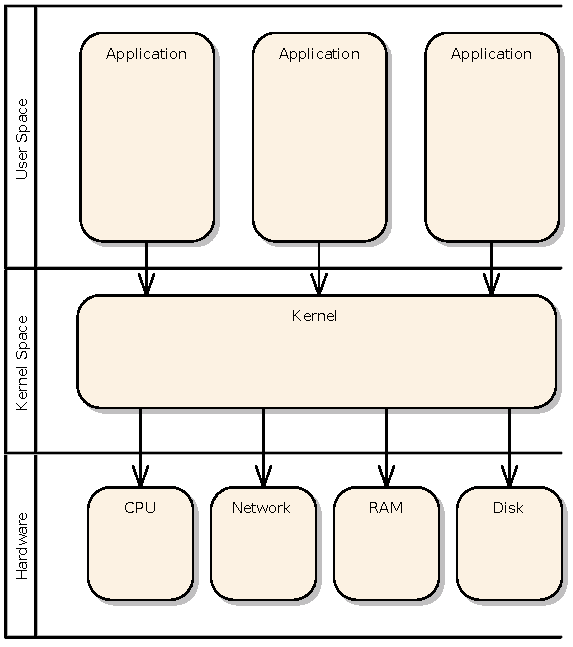
\includegraphics[scale=0.8]{images/kernel.pdf}
\caption{Linux Kernel}
\label{fig:kernel}
\end{wrapfigure}

Die \autoref{fig:kernel} zeigt, wie die unterschiedlichen Schichten miteinander kommunizieren. Eine Anwendung wird ausschliesslich im Benutzermodus (engl. User Space) ausgeführt. Durch Systemaufrufe werden Anfragen an den Kernel übermittelt. Dabei findet ein Kontextwechsel vom unprivilegierten in den privilegierten Modus statt. Der unprivilegierte Modus bezeichnet den Benutzermodus, in dem eine Applikation nur beschränkt über den Arbeitsspeicher verfügen kann und nur gewisse CPU-Befehlssätze ausgeführt werden können. Dies stellt sicher, dass eine Applikation gegenüber dem Rest des Systems abgekapselt betrieben wird und nicht darauf zugreifen kann. Nach dem Systemaufruf geht der Prozessor in den privilegierten Modus über und der Kernel trägt die Verantwortung, die Anfrage im Kernelmodus (engl. Kernel Space) zu verarbeiten. Der Kernelmodus weist im Gegensatz zum Benutzermodus keine Einschränkungen auf und hat deswegen auch Zugang zur Hardware und zum gesamten Arbeitsspeicher. Demzufolge dient der Kontextwechsel dazu, dass derjenige Programmcode, der nicht zum Kernel gehört, nur in einem unprivilegierten Modus ausgeführt werden kann.


\section{Unterschiede zwischen CISC- und RISC-CPUs}

Die Instruktionsarchitekturen der CPUs kann in zwei Gruppen unterteilt werden. Die CISC-Prozessoren (Custom Instruction Set Computer) mit sehr komplex und umfangreiche Instruktionsanweisungen und die RISC-Prozessoren (Reduced Instruction Set Computer) mit sehr primitive Instruktionsanweisungen.
\par
Der x86-Befehlssatz wurde durch den Intel 8086 Prozessor 1978 eingeführt und wurde somit zum Urvater moderne CISC-Prozessoren. Schon damals besitze dieser Prozessor ca. 120 Befehlssätze. Im Verlauf der Jahren zeichneten sich die CISC-Prozessoren mit immer mehr und komplexeren Befehlssätze aus. Dabei wurde immer beachtet das die Architektur, der neueren Modelle Rückwärtskompatibel, damit die Software ohne Anpassung auf neueren Prozessoren laufen kann. Die CISC-Architektur erlaubt es komplexe Instruktionen in einem Befehlssatz zu schreiben. Dabei wird der Befehlssatz von der CPU dekodiert und in einem oder mehreren Taktzyklen ausgeführt. Die Komplexität der Befehlssätze geht so weit das sogar Hardwareschleifen möglich werden. Ein anderes Merkmal der CISC-Prozessoren ist die geringe Anzahl der Register. Dafür kann ein Befehlssatz direkt die Anweisung haben, Daten von einer Speicherzelle im RAM zu einer andere zu transferiert ohne dabei auf ein Register angewiesen zu sein. Damit die immer komplexeren Befehlssätze dekodiert und in Instruktionen aufgeteilt werden können, besitzen die heutige CISC-Prozessoren sehr umfassende Steuerwerke. Allerdings bestehen die Steuerwerke nicht nur als Hardware Implementation, sondern besitzen teils innerhalb Microcode, die die Instruktionen an die ALU (Rechnerwerk) bilden kann.
\par
Bis Mitte der Achtziger war man der Meinung, dass grössere Leistung durch komplexere Hardware und die damit verbundene Anzahl an verfügbaren Befehlssätze möglich sei. Der Trend nahm aber ab. Zum einem wird heute kaum noch Programme in Assembler geschrieben. Und zum zweiten sind die gängigen Compiler so gebaut, dass sie nur etwa 20\% der Befehlssätze benötigen. Zu dem kommt das die komplexe Verarbeitungsstrukturen innerhalb des CISC-Prozessor die Elementaroperationen verlangsamen.
\par
Patterson, David A. und Sequin, Carlo H. prägten Ende der achtziger Jahre den Begriff RISC \cite{Patterson:1981:RIR:800052.801895}. Obwohl Prozessoren mit einfacher Architektur bereits schon viel früher existierten, schon deswegen weil die Technik noch nicht sehr ausgereift war und die Prozessoren nur eine begrenzte Anzahl an Instruktionen verarbeiten konnten. RISC-Prozessoren Zeichnen sich durch eine Load-and-Store-Architektur, höhere Menge an Universelle-Registern und auf die Begrenzung auf die Elementarinstruktionen. Der Begriff "Load and Store" meint, dass Daten immer über Registern geladen und gespeichert werden müssen. Es ist also bei dieser Architektur nicht möglich die Daten von einer Speicherzelle im RAM zu einer andere zu transferieren ohne sie zuerst in einem Register zwischen zu speichern. Es benötigt bei diesem Vorgehen mindestens zwei Taktzyklen, den ersten zum Laden in einem Zwischenregister und den zweiten zum abspeichern in einer andere Speicherzelle. Durch die grössere Anzahl an Registern muss dafür ein RISC-Prozessor weniger auf dem Speicher zurückgreifen als ein CISC-Prozessor.
\par
Die frühere klassische Trennung der CISC- und RISC-Prozessoren wird immer wie kleiner. Die Entwicklung der CISC-Prozessoren hat sich stark nach den RISC-Prozessoren ausgerichtet. Da sie intern praktisch mit einer RISC-Struktur und einer hochentwickelten Vorverarbeitungsstufe ausgestattet sind. Bereits der Pentium Pro war mit einem RISC-Kern ausgestattet und die x86-Schnittstelle nach aussen, war so zu sagen ein vorgeschalteten x86-Emulator.



%\section{Energy Storage in a Capacitor}
%Grundlage Technische Informatik Kap. Halbleitertechnik lesen!



\section{Relevanz für das Experiment}

Prozessoren sind als elektronische Schaltkreise realisiert. Die Schaltkreise werden durch die Halbleitertechnologie hergestellt. Die Millionen von witzigen Transistoren, die ein Prozessor beinhaltet, werden zu logischen Bausteinen verdrahtet.
\par
In dieser Arbeit ist die Funktionsweise der ALU relevant. Wir wissen, dass die ALU eine Reihe von Anweisungen erhält und somit jeden erdenklichen Algorithmus ausführen kann. Im Rahmen dieser Arbeit wird eine Methode entwickelt, um den Energieverbrauch einer einzelnen Anweisung der ALU messen können.


